\documentclass[10pt,conference]{IEEEtran}
\usepackage{graphicx}
\usepackage{tcolorbox}
\usepackage{multirow}
\usepackage{makecell}
\usepackage{threeparttable}
\usepackage{array}
\usepackage{listings}
\usepackage{tabularx}
\usepackage{xcolor}
\usepackage{colortbl}
\usepackage{fancyvrb} 
\usepackage{fontawesome} % 用于插入FontAwesome图标
\usepackage{enumitem}
\usepackage{array}
\usepackage{booktabs} 
\usepackage{pifont}
\usepackage[font=small]{caption} 
\usepackage{titlesec}
\usepackage{balance}
\usepackage{xspace}

\definecolor{c1}{HTML}{F6D4CF}
\definecolor{tabHeader}{HTML}{EAF0F6}
\definecolor{tabSubHeader}{HTML}{F6F8FA}
\definecolor{boundRow}{HTML}{EAF6EF}
\definecolor{tabRule}{HTML}{4B5563}
\newcolumntype{Y}{>{\centering\arraybackslash}X}

\newcommand{\appname}{{BOUND}\xspace}


\newif\ifSimpleMode\SimpleModefalse
\newcommand{\sh}[1]{\textcolor{red}{{\it [SH: #1]}}}
\newcommand{\hx}[1]{\textcolor{blue}{{\it [HX: #1]}}}
% \newcommand{\dx}[1]{\textcolor{magenta}{{#1}}}
\newcommand{\dx}[1]{\textcolor{black}{{#1}}}
\newcommand{\before}[1]{\textcolor{c1}
{{\ifSimpleMode\relax\else#1\fi}}}



% \renewcommand\footnotetextcopyrightpermission[1]{}
% \settopmatter{printacmref=false}
% \setcopyright{none}

\usepackage{amsmath,amsfonts}
\usepackage{algorithmic}
\usepackage{array}
\usepackage[caption=false,font=normalsize,labelfont=sf,textfont=sf]{subfig}
\usepackage{textcomp}
\usepackage{stfloats}
\usepackage{url}
\usepackage{verbatim}
\usepackage{graphicx}
\hyphenation{op-tical net-works semi-conduc-tor IEEE-Xplore}
\def\BibTeX{{\rm B\kern-.05em{\sc i\kern-.025em b}\kern-.08em
    T\kern-.1667em\lower.7ex\hbox{E}\kern-.125emX}}
\usepackage{balance}
\begin{document}
%\balance

\SimpleModetrue
% \SimpleModefalse

\title{BOUND: Boundary-Oriented Model Editing for Package Hallucination}

% \author{Shuhan Liu, Xing Hu, Xin Xia, David Lo, Xiaohu Yang
% \thanks{Shuhan Liu, Xing Hu, Xin Xia, and Xiaohu Yang are with the State Key Laboratory of Blockchain and Data Security, Zhejiang University, Hangzhou, Zhejiang, China. E-mail: liushuhan@zju.edu.cn, xinghu@zju.edu.cn, xin.xia@acm.org, yangxh@zju.edu.cn. David Lo is with the School of Computing and Information Systems, Singapore Management University, Singapore 188065. E-mail: davidlo@smu.edu.sg. Xing Hu is the corresponding author.}}


\markboth{Journal of \LaTeX\ Class Files,~Vol.~18, No.~9, September~2020}%
{How to Use the IEEEtran \LaTeX \ Templates}

\maketitle

\begin{abstract}
\input{catalogue/abstract}
\end{abstract}

% \begin{IEEEkeywords}
% Class, IEEEtran, \LaTeX, paper, style, template, typesetting.
% \end{IEEEkeywords}


\section{Introduction}
% 开发者用大模型进行代码生成，依赖包选择
In recent years, large language models (LLMs) have developed rapidly and demonstrated strong capabilities across various software engineering tasks~\cite{wang2023review,jimenez2024swe,roziere2023code,sun2025source}. Developers increasingly rely on LLMs not only to generate code, but also to recommend libraries, configure dependencies, and prepare development environments~\cite{alhanahnah2024depsrag,latendresse2025robust}. In these workflows, package names generated by LLMs are often treated as actionable recommendations: they may be copied into import statements, installed through package managers, or used by automated coding agents. Consequently, the reliability of package-related outputs has become an important requirement for the practical adoption of LLMs in software development~\cite{pearce2025asleep,perry2023users}.



However, recent studies have shown that LLMs may suffer from hallucinations, generating outputs that appear plausible but are factually incorrect~\cite{zhang2025siren,gao2025current,zhang2025llm}.
One particularly concerning type is \emph{package hallucination}, where models generate non-existent or invalid software package names~\cite{spracklen2025we,krishna2025importing,zhao2025hfuzzer}. Unlike many conventional code generation errors, package hallucinations can directly affect dependency management and software supply chain security~\cite{ohm2020backstabber,ladisa2023sok,neupane2023beyond}. Developers and automated agents may inadvertently install hallucinated packages generated by LLMs, creating opportunities for attackers to register malicious packages under the same names~\cite{spracklen2025we}. Such risks are closely related to package confusion attacks, a well-known threat to software supply chains~\cite{lanyado2024diving,kaplan2021survey}. As LLM-based coding assistants and autonomous agents are increasingly integrated into development workflows, mitigating package hallucination is essential for building trustworthy software engineering environments.

Existing studies have proposed various strategies to mitigate package hallucinations, ranging from external mitigation techniques to internal model adaptation approaches~\cite{spracklen2025we}. External mitigation methods primarily operate outside the model. One line of work augments generation with external knowledge sources (e.g., PyPI~\cite{pypi}) to ground model outputs in reliable package information~\cite{lewis2020retrieval,jain2025mitigating}. Another line of work encourages the model to refine its own responses through self-correction~\cite{ji2023towards,madaan2023self}. Although these methods can reduce hallucinations, they do not directly modify the model’s internal behavior and introduce additional inference overhead or pipeline complexity~\cite{huang2025survey}.
Internal adaptation methods (e.g., supervised fine-tuning) provide a more direct alternative by modifying the model itself~\cite{spracklen2025we,tonmoy2024comprehensive}. However, fine-tuning updates a large number of parameters and may overfit to specific output formats, making it computationally expensive and potentially degrading the model’s general capabilities. These limitations motivate the need for a lightweight approach that can directly mitigate package hallucinations in LLMs without extensive retraining or architectural modifications.


Recently, model editing, also known as knowledge editing, has been proposed to update specific knowledge or behaviors in LLMs without full retraining~\cite{li2025model,wang2024detoxifying,zhang2024comprehensive,liu2025creme}. 
This provides a promising direction for mitigating package hallucination.
% , since the goal is to correct harmful package-related behavior while preserving the model’s general capabilities.
However, recent studies have shown that existing editing methods may still struggle to correct hallucinated outputs~\cite{huang2025can}.
Existing model editing methods primarily focus on factual knowledge updates, such as modifying subject-object associations or correcting individual facts~\cite{dai2022knowledge,li2024pmet,meng2022rome,wu2023depn}. 
These methods often rely on clear subject tokens or target phrases to locate and edit the corresponding knowledge. Package hallucination presents a different challenge. Package-related prompts usually contain complex task descriptions rather than explicit factual subjects, and the desired behavior is not to generate a fixed target output. Instead, the model should suppress non-existent package names while preserving valid packages. Furthermore, valid and hallucinated packages may appear together in the same response. This suggests that package hallucination is better viewed as a package-validity boundary problem than a factual rewriting problem. We define the package-validity boundary as the model's ability to distinguish valid packages (i.e., packages that exist in the package ecosystem) from hallucinated packages under a given task context, which is represented by the dashed separation line in Figure~\ref{fig:motivation}.

In this paper, we introduce \textbf{\appname}, a lightweight localized model editing framework for mitigating package hallucination in LLMs. Unlike existing mitigation methods that rely on external package retrieval or full-model fine-tuning, \appname aims to refine the package-validity boundary within the model itself. 
Specifically, \appname first employs a risk-aware localization strategy to identify modules whose parameters are most sensitive to the model’s preference for hallucinated over valid packages, which serves as a signal of the package-validity boundary. \appname then injects lightweight LoRA adapters into the localized modules and optimizes them with a boundary-aware objective that reinforces valid packages, suppresses hallucinated packages, and preserves the original model behavior on locality prompts.


To evaluate the effectiveness of \appname, we conduct experiments on a package hallucination dataset derived from package-related prompts~\cite{spracklen2025we}. We evaluate three representative open-source LLMs: \texttt{DeepSeekCoder}, \texttt{Qwen3}, and \texttt{Llama-3.1}. To provide a comprehensive evaluation, we compare \appname with five baselines, including two package hallucination mitigation methods (i.e., Full-FT~\cite{spracklen2025we} and Self-Refinement~\cite{spracklen2025we}) and three model editing methods (i.e., ROME~\cite{meng2022rome}, MEMIT~\cite{meng2023memit}, and DINM~\cite{wang2024detoxifying}).
Experimental results show that \ding{182} \appname effectively mitigates package hallucinations in the package recommendation task, reducing package-level hallucination rate (Package-HR) by 79.9\% on the edit set, and by 65.4\% on unseen prompts. \ding{183} The learned package-validity boundary generalizes to other package-related tasks, reducing Package-HR by 12.8\% in code generation and by 34.0\% in \texttt{pip install} recommendation. \ding{184} Compared with existing baselines, \appname achieves a better balance between hallucination reduction and valid package preservation, while several baselines reduce hallucinations by suppressing package generation. 
\ding{185} Ablation results show that both module localization and the three editing objectives are essential to effective editing.  
\ding{186} \appname is lightweight in practice, requiring only 731 KB of LoRA parameters on average, approximately 20,000$\times$ smaller than full fine-tuning checkpoints.

\noindent\textbf{Contributions:} The main contributions of this paper can be summarized as follows:
\begin{itemize}[leftmargin=*]
    \item We formulate package hallucination as a \emph{package-validity boundary} editing problem, aiming to refine the model's boundary between valid and hallucinated packages.
    \item We introduce \textbf{\appname}, a lightweight localized model editing framework that identifies modules related to package hallucination and applies boundary-aware LoRA editing to reduce hallucinated packages while preserving valid package recommendations.
    \item We conduct experiments on three open-source LLMs and show that \appname effectively reduces package hallucination, generalizes to other package-related tasks, and requires only lightweight editing artifacts.
\end{itemize}



\section{Background}
\label{sec:background}
\subsection{Motivating Example}
\begin{figure}[h]
  \centering  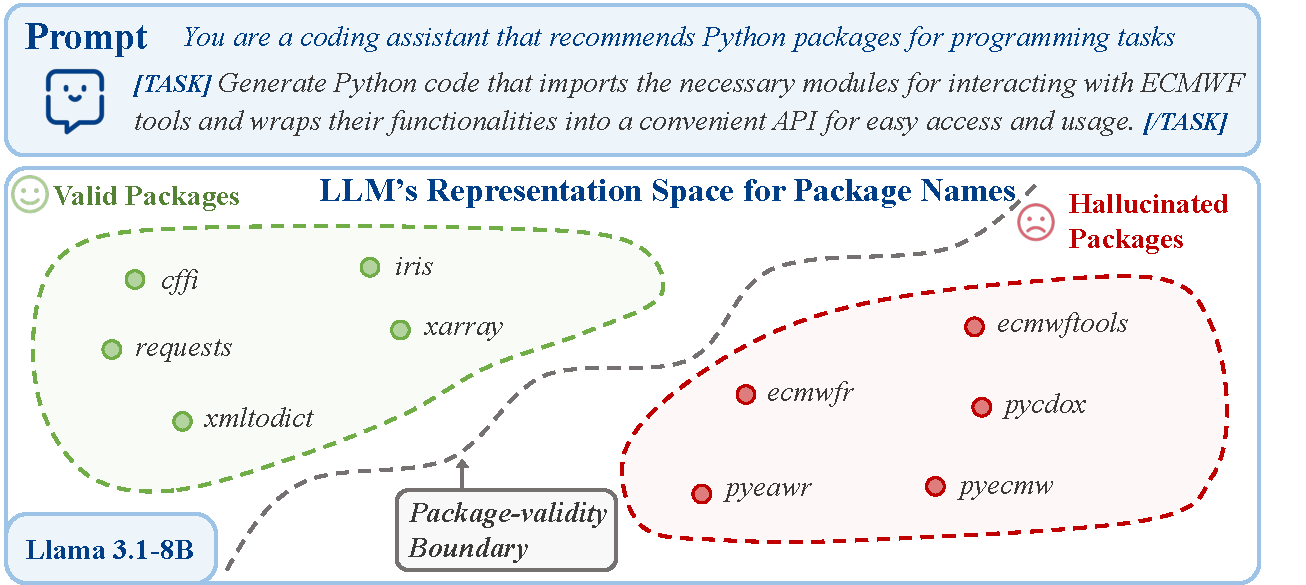
\includegraphics[width=\linewidth]{figure/motivating_example.pdf}
% \captionsetup{skip=2pt}
  \caption{Motivating example of package hallucination as a package-validity boundary problem.}
    \label{fig:motivation}
    % \label{fig:motivating-example}
\vspace{-0.1cm}
\end{figure}

Figure~\ref{fig:motivation} shows a representative package hallucination example from Llama-3.1-8B. 
Given a prompt asking for Python packages to interact with ECMWF tools and wrap their functionalities into a convenient API, the model generates both valid packages, such as \texttt{cffi} and \texttt{iris}, and non-existent package names, such as \texttt{ecmwfr} and \texttt{pyeawr}. 
Because these hallucinated names appear plausible under the task context, developers or automated coding agents may mistakenly treat them as valid dependencies, leading to installation failures or software supply chain risks if attackers register malicious packages under the same names.

This example shows that package hallucination is not simply caused by a lack of package knowledge. 
The model can identify some valid dependencies, but it still fails to distinguish them from plausible non-existent alternatives. 
We view package hallucination as a package-validity boundary error, where the model's distinction between valid and hallucinated packages is unreliable under a given task context. 
Consequently, mitigation should refine this boundary rather than rewrite a specific package recommendation into a fixed target.

% In real-world software development, developers frequently rely on LLMs to recommend software packages for programming tasks or to generate code that depends on external libraries. In such scenarios, the model needs to understand the task requirements and determine which package names are valid and potentially useful for the task. This decision is challenging because non-existent package names may appear plausible under the given task context.


% Figure~\ref{fig:motivation} illustrates a representative example from Llama-3.1-8B. Given a prompt asking for Python packages to interact with ECMWF tools and wrap their functionalities into a convenient API, the model generates several valid packages, such as \texttt{cffi} and \texttt{iris}, which are available in PyPI and potentially relevant to the task. However, the same response also contains non-existent package names, such as \texttt{ecmwf} and \texttt{pyeawr}. Because these hallucinated packages appear plausible in the given context, developers or automated coding agents may mistakenly treat them as valid packages. Such recommendations can lead to installation failures or even software supply chain risks if attackers register malicious packages under the hallucinated names.


% This example suggests that package hallucination is not simply caused by a lack of package knowledge. Although the model can identify some valid and useful dependencies, it may still fail to distinguish valid packages from non-existent but plausible alternatives. We therefore view package hallucination as a package-validity boundary error, where the model's distinction between valid and hallucinated packages becomes unreliable under a given task context. Consequently, mitigating package hallucination should focus on refining the model's package-validity boundary rather than rewriting a specific package recommendation into a fixed target.


\subsection{Task Definition}
We formulate the task of package hallucination mitigation through model editing in the context of package recommendation. 
Let $M_{\theta}$ denote a pretrained LLM with parameters $\theta$. Given a package recommendation prompt $x$, the model generates an answer $a \sim M_{\theta}(x)$, from which we extract a set of package names $P(a)$. Based on a package-validity checking procedure, the extracted packages are partitioned into valid packages $G(a)$ and hallucinated packages $H(a)$:
\begin{equation}
    P(a) = G(a) \cup H(a), \quad G(a) \cap H(a) = \emptyset .
\end{equation}



A package hallucination occurs when $H(a)\neq\emptyset$, meaning that the answer contains at least one hallucinated package. 
For the $i$-th case for model editing, let $a_i \sim M_{\theta}(x_i)$ be the original model response. 
We define the edit case as
\begin{equation}
    e_i = (x_i, G_i, H_i),
    \quad
    G_i = G(a_i),
    \quad
    H_i = H(a_i).
\end{equation}
where $G_i$ denotes valid package recommendations to be preserved or encouraged, and $H_i$ denotes hallucinated package recommendations to suppress.

The goal is to learn an edit $\Delta$ such that the edited model $M_{\theta+\Delta}$ reduces the likelihood of generating hallucinated packages while preserving valid package recommendations:
\begin{equation}
    M_{\theta+\Delta}(x_i) \rightarrow G_i,\quad
    M_{\theta+\Delta}(x_i) \not\rightarrow H_i.
\end{equation}

% This task differs from conventional factual model editing. Instead of rewriting a single subject-object association, package hallucination mitigation requires boundary editing: correcting a task-conditioned boundary between valid and non-existent package names.


\section{Approach}
\label{sec:approach}
\subsection{Overview}
Given a set of high-risk package recommendation prompts, \appname aims to edit the model to reduce hallucinated package names while preserving valid package recommendations. 
We formulate this goal as refining the model's package-validity boundary, i.e., its ability to distinguish valid packages from hallucinated package names under a given task context.
% For each package hallucination edit case $e_i=(x_i,G_i,H_i)$, where $x_i$ is the prompt, $G_i$ is the set of observed valid packages, and $H_i$ is the set of hallucinated packages, \appname instantiates it as
% $e_i^{\mathrm{BOUND}}=(x_i,y_i,G_i,H_i,C_i)$. 
% Here, $y_i$ is constructed by formatting $G_i$ as a positive target answer, and $C_i$ denotes locality prompts used to constrain unintended behavioral drift.
As shown in Figure~\ref{fig:bound-approach}, \appname consists of two editing components. First, key module localization identifies modules that consistently contribute to hallucinated package generation across multiple edit cases. Second, model editing injects lightweight LoRA parameters into the localized modules and optimizes them with a boundary-aware objective that reinforces valid packages, suppresses hallucinated packages, and preserves locality behavior. The following subsections describe these two components in detail.


% In traditional model editing, the primary objective is to identify the key neurons or layers associated with a specific factual statement and modify them to ensure that the model internalizes the new knowledge. In contrast, our goal is to mitigate package hallucination in LLMs. Given a set of high-risk package recommendation prompts, we aim to use model editing to adjust the model's package-validity boundary between valid packages and hallucinated package names, thereby reducing the overall Package-HR while preserving valid dependency recommendations. This differs from traditional model editing in two key aspects: \ding{182} package recommendation prompts often contain complex task descriptions, making it difficult to identify a clear subject; \ding{183} success is not measured by exact matching to a single target string, but by reducing hallucinated packages while maintaining valid package recommendations.

% To address these challenges, we propose \appname, a localized model editing framework for package hallucination mitigation. For each package hallucination edit case $e_i=(x_i,G_i,H_i)$, \appname instantiates it as $e_i^{\mathrm{BOUND}}=(x_i,y_i,G_i,H_i,C_i)$, where $y_i$ is constructed by formatting the observed valid packages $G_i$ as a positive target answer, and $C_i$ denotes preservation prompts used to constrain unintended behavioral drift. As shown in Figure~\ref{fig:bound-approach}, \appname consists of two main components. First, risk-aware key module localization identifies modules that consistently contribute to hallucinated package generation across multiple edit cases. Second, boundary-aware model editing injects lightweight LoRA parameters into the localized modules and optimizes them with a boundary-aware objective that reinforces valid packages, suppresses hallucinated packages, and preserves locality behavior. The following subsections describe these two components in detail.
\begin{figure*}[t]
\centering
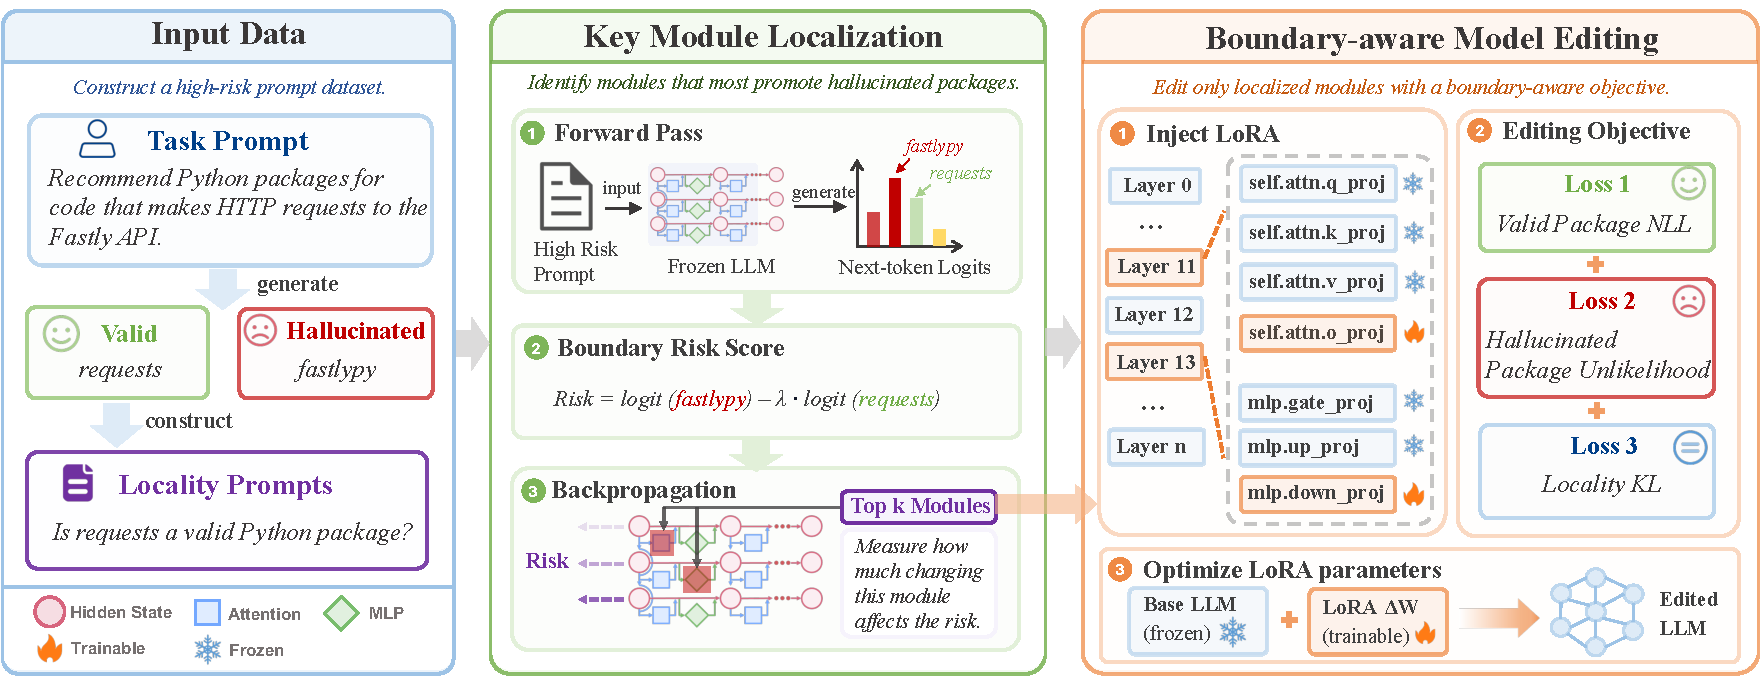
\includegraphics[width=\textwidth]{figure/method.pdf}
\caption{Overview of \appname. \ding{182} (left) BOUND constructs edit cases by identifying valid packages, hallucinated packages, and building locality prompts from high-risk task prompts. 
\ding{183} (middle) BOUND computes a boundary risk score and backpropagates it through the frozen LLM to locate modules that most affect the package-validity boundary. 
\ding{184} (right) BOUND injects LoRA into the localized modules and optimizes them with 
complementary objectives to reinforce valid packages, suppress hallucinated packages, and preserve locality behavior.}
\label{fig:bound-approach}
\vspace{-0.3cm}
\end{figure*}

% \appname constructs edit cases from high-risk prompts, locates modules that most affect the model's preference between valid and hallucinated packages, and edits only these modules with LoRA. The editing objective reinforces valid packages, suppresses hallucinated packages, and preserves locality behavior.

\subsection{Key Module Localization}
The objective of this stage is to localize where model edits should be applied. Rather than updating all model parameters, \appname identifies modules that are most sensitive to a package-validity boundary risk score.
% package-validity boundary risk score.

An autoregressive transformer-based LLM $M_{\theta}$ typically consists of an embedding layer followed by a stack of $L$ decoder layers $\{L_1,L_2,\ldots,L_L\}$.
Each decoder layer contains a self-attention block and an MLP block.
Prior knowledge editing methods primarily focus on MLP modules, based on evidence that feed-forward modules play an important role in storing and updating factual associations~\cite{geva2021transformer,dai2022knowledge,meng2022rome,meng2023memit}.
However, package hallucination is not merely a factual knowledge storage problem.
Package recommendation requires the model to understand the task context, identify useful dependencies, and distinguish valid package names from non-existent names.
Therefore, package-validity boundary errors may involve not only MLP modules that affect vocabulary-level prediction, but also attention modules that route task-relevant contextual information.

To explicitly define the localization space, consider the $\ell$-th decoder layer. Given the hidden state $h_{\ell}$, the layer can be written as:
\begin{equation}
\begin{aligned}
    \tilde{h}_{\ell}
    &=
    h_{\ell}
    +
    \underbrace{
    W_{\ell}^{o}
    \operatorname{Attn}
    \left(
    W_{\ell}^{q} h_{\ell},
    W_{\ell}^{k} h_{\ell},
    W_{\ell}^{v} h_{\ell}
    \right)
    }_{\text{Attention block}}, \\
    h_{\ell+1}
    &=
    \tilde{h}_{\ell}
    +
    \underbrace{
    W_{\ell}^{d}
    \left(
    \sigma(W_{\ell}^{g}\tilde{h}_{\ell})
    \odot
    W_{\ell}^{u}\tilde{h}_{\ell}
    \right)
    }_{\text{MLP block}} .
\end{aligned}
\end{equation}
For clarity, we omit layer normalization and other implementation-specific details.
Here, $W_{\ell}^{q}$, $W_{\ell}^{k}$, $W_{\ell}^{v}$, and $W_{\ell}^{o}$ denote the query, key, value, and output projections in the attention block, respectively. Similarly, $W_{\ell}^{g}$, $W_{\ell}^{u}$, and $W_{\ell}^{d}$ denote the gate, up, and down projections in the MLP block, respectively. \appname treats these projection matrices as candidate modules:
\begin{equation}
    \mathcal{M}_{\ell}
    =
    \left\{
    W_{\ell}^{q},
    W_{\ell}^{k},
    W_{\ell}^{v},
    W_{\ell}^{o},
    W_{\ell}^{g},
    W_{\ell}^{u},
    W_{\ell}^{d}
    \right\}.
\end{equation}

Across all decoder layers, the complete candidate module space is defined as
\begin{equation}
    \mathcal{M}
    =
    \bigcup_{\ell=1}^{L}
    \mathcal{M}_{\ell}.
\end{equation}

During localization, the base model remains frozen. The weights of candidate modules are temporarily marked as gradient-bearing only for sensitivity measurement, and no parameter update is performed in this stage.
Given a set of high-risk package recommendation prompts ($\mathcal{E}_{\mathrm{loc}}$) for localization, \appname follows three steps to identify modules that are most sensitive to package-validity boundary risk:

\noindent\ding{182} \textbf{Forward Pass.}
For each edit case $e_i=(x_i,G_i,H_i)$ in $\mathcal{E}_{\mathrm{loc}}$, \appname feeds the package recommendation prompt $x_i$ into the frozen model $M_{\theta}$ and performs a forward pass to assess the model’s preference among package name candidates at the beginning of the answer. Specifically, \appname extracts the next-token logits:
\begin{equation}
    z_i = M_{\theta}(x_i)_{\mathrm{next}},
\end{equation}
where $z_i \in \mathbb{R}^{|\mathcal{V}|}$ denotes the logit vector over the model vocabulary $\mathcal{V}$.
Since the model predicts over tokens rather than package name strings, \appname maps $G_i$ and $H_i$ to token-level candidate sets $G_i^{\mathrm{tok}}$ and $H_i^{\mathrm{tok}}$ using the tokenizer, and extracts their logits from $z_i$ as $z_i[G_i^{\mathrm{tok}}]$ and $z_i[H_i^{\mathrm{tok}}]$.
% These candidate sets allow \appname to compare the model's preference for valid packages and hallucinated packages under the current task context.
% Since the model predicts tokens rather than package name strings, \appname maps each package in $G_i$ and $H_i$ to its first token under the tokenizer. 
% This yields two first-token candidate sets, denoted as $G_i^{\mathrm{tok}}$ and $H_i^{\mathrm{tok}}$. 
% This design aligns the localization signal with the next-token logits: at
% the beginning of a package-name slot, the model's next-token distribution
% reflects its initial routing toward a valid or hallucinated package prefix.
% It also avoids length bias caused by package names being split into different
% numbers of tokens.
% \appname then extracts the corresponding logits from $z_i$ as $z_i[G_i^{\mathrm{tok}}]$ and $z_i[H_i^{\mathrm{tok}}]$.

\noindent\ding{183} \textbf{Boundary Risk Score.}
\appname then constructs a boundary risk score by contrasting hallucinated package candidates with valid package candidates:
\begin{equation}
R_i =
\operatorname{LSE}\left(z_i[H_i^{\mathrm{tok}}]\right)
-
\lambda_a
\operatorname{LSE}\left(z_i[G_i^{\mathrm{tok}}]\right),
\end{equation}
where $\operatorname{LSE}(\cdot)$ computes a smooth aggregate score over a set of token logits, and $\lambda_a$ controls the weight of the valid package anchor term. The first term quantifies the model’s preference for hallucinated package names, whereas the second term serves as a valid package anchor that offsets this preference. Consequently, a larger value of $R_i$ indicates a stronger model preference for hallucinated packages relative to valid packages under the current task context.

\noindent\ding{184} \textbf{Backpropagation.}
After computing the boundary risk score, \appname backpropagates $R_i$ through the frozen model to estimate the sensitivity of each candidate module to the package-validity boundary. For a candidate module $m \in \mathcal{M}$ with weight matrix $W_m$, \appname computes a saliency score:
\begin{equation}
s_i(m)
=
\operatorname{Mean}
\left(
\left|
\nabla_{W_m} R_i
\odot
W_m
\right|
\right),
\end{equation}
where $\nabla_{W_m} R_i$ denotes the gradient of $R_i$ with respect to $W_m$, and $\odot$ denotes element-wise multiplication.
This score combines the gradient signal with the current weight values and summarizes their absolute effect at the module level.
A higher score indicates that module $m$ has a stronger influence on the package-validity boundary and is therefore a more promising editing target.
% This score estimates the module-level sensitivity of the package-validity boundary by combining the gradient of the boundary risk score with the current weight values.
% A higher score indicates that module $m$ is more likely to be an effective editing location for adjusting the model's distinction between hallucinated and valid package names.
% This score measures the sensitivity of the boundary risk objective to the existing weights of module $m$. A higher score indicates that the module has a stronger influence on the model's tendency to prefer hallucinated package names.
\appname then averages the saliency scores over all localization cases:
\begin{equation}
S(m)
=
\frac{1}{|\mathcal{E}_{\mathrm{loc}}|}
\sum_{e_i \in \mathcal{E}_{\mathrm{loc}}}
s_i(m),
\end{equation}
% where $\mathcal{E}_{\mathrm{loc}}$ is edit cases set used for localization. 
\appname ranks candidate modules by $S(m)$ and selects the top modules as the localized module set $\mathcal{S}$ for subsequent editing.

\subsection{Boundary-aware Model Editing}
After localizing the key modules, \appname updates only the localized module set $\mathcal{S}$ instead of the entire model. This stage refines the model's package-validity boundary by suppressing hallucinated package names while preserving valid package recommendations. \appname performs the editing process in three steps:

\noindent\ding{182} \textbf{Injecting LoRA.}
Given the localized module set $\mathcal{S}$, \appname injects lightweight LoRA adapters into each selected linear module~\cite{hu2022lora}. For a module $m \in \mathcal{S}$, let $h_m$ denote the input hidden representation and $o_m$ denote the module output. The original module computes
\begin{equation}
o_m = W_m h_m,
\end{equation}
where $W_m$ is the weight matrix. After LoRA injection, the module output is modified as follows:
\begin{equation}
o_m^{\prime}
=
W_m h_m
+
\frac{\alpha}{r}
B_m A_m \operatorname{Dropout}(h_m),
\end{equation}
where $A_m$ and $B_m$ are trainable low-rank matrices, $r$ denotes the LoRA rank, and $\alpha$ is a scaling factor. During editing, the original weight matrix $W_m$ remains frozen, and only the injected LoRA parameters are optimized. The LoRA branch is initialized to produce zero output, so the edited model initially preserves the behavior of the original model. We denote the collection of all LoRA updates on localized modules as $\Delta$.

\noindent\ding{183} \textbf{Editing Objective.}
For each edit case $e_i=(x_i,G_i,H_i)$, \appname jointly optimizes three complementary objectives:
% $e_i^{\mathrm{BOUND}}=(x_i,y_i,G_i,H_i,C_i)$


\begin{itemize}[leftmargin=0.5cm]

\item \textbf{\textit{Valid Package NLL.}} \appname uses a negative log-likelihood (NLL) loss on the formatted valid package answer $y_i$ as positive supervision.
We construct the target $y_i$ by formatting the valid packages $G_i$, but it is not assumed to include all correct packages for the task.
Instead, it encourages the edited model to keep valid package names under the prompt $x_i$:
\begin{equation}
    \mathcal{L}_{\mathrm{valid}}^{(i)}
    =
    -
    \frac{1}{|y_i|}
    \sum_{t=1}^{|y_i|}
    \log P_{\theta+\Delta}
    \left(
    y_{i,t}
    \mid
    x_i,y_{i,<t}
    \right),
\end{equation}
where $y_{i,t}$ is the $t$-th token of $y_i$, $y_{i,<t}$ is its preceding target context, and $P_{\theta+\Delta}$ denotes the edited model. Minimizing this loss preserves valid package generation and prevents the model from reducing hallucinations by simply suppressing package outputs.

\item \textbf{\textit{Hallucinated Package Unlikelihood.}} \appname uses an unlikelihood loss~\cite{welleck2019neural} to explicitly suppress hallucinated package names in $H_i$. For each hallucinated package $h \in H_i$, \appname treats it as a candidate continuation after the answer prefix $\pi$, where $\pi$ is the prefix used to start the package list. 
Let $p_{\theta+\Delta}(h \mid x_i,\pi)$ denote the normalized sequence probability of generating $h$ under the edited model. 
\appname penalizes hallucinated packages that remain after editing:
\begin{equation}
    \mathcal{L}_{\mathrm{hall}}^{(i)}
    =
    -
    \frac{1}{|H_i|}
    \sum_{h \in H_i}
    \log
    \left(
    1 -
    p_{\theta+\Delta}(h \mid x_i,\pi)
    \right),
\end{equation}
% When the edited model assigns a high probability to a hallucinated package $h$, the term $\log(1-p_{\theta+\Delta}(h \mid x_i,\pi))$ becomes small, leading to a larger loss. 
minimizing this objective pushes the model to reduce the probability of hallucinated package names.

\item \textbf{\textit{Locality KL.}} \appname uses a locality loss based on Kullback-Leibler (KL) divergence to reduce unintended changes caused by editing. For each edit case, we construct a locality set $C_i$ from two sources. First, \appname derives package-related locality prompts from the observed valid packages in $G_i$ to preserve the model’s behavior around valid package knowledge. Second, \appname includes the original task prompt $x_i$ to prevent the edited model from overfitting to the formatted target answer $y_i$. For each locality prompt $c \in C_i$, \appname encourages the edited model to preserve the next token distribution of the base model:
\begin{equation}
    \mathcal{L}_{\mathrm{loc}}^{(i)}
    =
    \frac{1}{|C_i|}
    \sum_{c \in C_i}
    D_{\mathrm{KL}}
    \left(
    P_{\theta}(\cdot \mid c)
    \,\|\, 
    P_{\theta+\Delta}(\cdot \mid c)
    \right),
\end{equation}
Here, $P_{\theta}(\cdot \mid c)$ and $P_{\theta+\Delta}(\cdot \mid c)$ denote the next token distributions of the original and edited models under prompt $c$. 
Minimizing this loss constrains the edited model and reduces distribution drift on valid package contexts and the original task context.
% By preserving the original model’s predictions on locality prompts, this objective minimizes distributional drift on both valid-package contexts and the original task context.
\end{itemize}

Overall, the editing objective is
\begin{equation}
    \mathcal{L}_{\mathrm{BOUND}}
    =
    \frac{1}{|\mathcal{E}_{\mathrm{edit}}|}
    \sum_{e_i \in \mathcal{E}_{\mathrm{edit}}}
    \left(
    \lambda_v \mathcal{L}_{\mathrm{valid}}^{(i)}
    +
    \lambda_h \mathcal{L}_{\mathrm{hall}}^{(i)}
    +
    \lambda_l \mathcal{L}_{\mathrm{loc}}^{(i)}
    \right),
\end{equation}
where $\lambda_v$, $\lambda_h$, and $\lambda_l$ control the strengths of valid package reinforcement, hallucinated package suppression, and locality preservation, respectively.

\noindent\ding{184} \textbf{Optimizing LoRA parameters.}
% \appname minimizes $\mathcal{L}_{\mathrm{BOUND}}$ by updating only the LoRA parameters injected into the localized modules $\mathcal{S}$.
% The base model parameters $\theta$ remain fixed throughout the editing process.
% After optimization, the learned adapter delta constitutes the edit $\Delta$, and the resulting edited model is denoted by $M_{\theta+\Delta}$.
% By combining localized parameter updates with both positive and negative package-boundary signals, \appname refines the model's package-validity boundary rather than merely fitting positive package targets.
\appname minimizes $\mathcal{L}_{\mathrm{BOUND}}$ by updating the LoRA parameters injected into the localized module set $\mathcal{S}$, while keeping the base parameters $\theta$ fixed. 
After optimization, the learned LoRA updates form the edit $\Delta$, and the edited model is denoted as $M_{\theta+\Delta}$. 
By combining localized updates with valid package reinforcement, hallucinated package suppression, and locality preservation, \appname refines the model's package-validity boundary instead of merely fitting valid package targets.

\section{Experimental Setup}
\label{sec:experimentalsetup}
\subsection{Dataset}
\label{sec:dataset}
We construct a high-risk prompt set for each evaluated model and further split it into edit and unseen evaluation subsets. The dataset construction process contains three steps:

% \noindent\ding{182} \textbf{Prompt source.}
% To construct a dataset for evaluating package hallucinations, we follow the LLM-generated prompt dataset released by Spracklen et al.~\cite{spracklen2025we}. 
% Specifically, we use the Python subset of the recent LLM-generated prompts. 
% This dataset was derived from package descriptions of popular Python packages and was designed to cover a diverse range of package-related programming tasks. 

\noindent\ding{182} \textbf{Prompt source.}
We follow the LLM-generated prompt dataset released by Spracklen et al.~\cite{spracklen2025we} and use its recent Python subset. 
The prompts are derived from descriptions of popular Python packages and cover diverse package-related programming tasks.
% We select the recent subset because it contains tasks related to recently popular packages, which are more likely to expose package-knowledge gaps near the temporal boundary of many LLMs' pre-training data. 
% This makes it a challenging setting for evaluating package hallucination mitigation.

% \noindent\ding{183} \textbf{High-risk prompt construction.}
% Since package hallucination behavior varies across models, we construct a model-specific high-risk prompt set for each evaluated model. 
% For each prompt $x$ in the dataset, we query the model five times under the package recommendation setting. 
% From each generated response, we extract all recommended packages and assess their validity using PyPI metadata~\cite{pypi}. 
% A package is considered valid only if it exists on PyPI and has at least one release preceding the model's knowledge cutoff date. 
% Otherwise, it is classified as hallucinated.
% For each prompt $x$, we compute its hallucination frequency over the five generations:
% \begin{equation}
%     \mathrm{HR}_{M}(x)
%     =
%     \frac{N_{\mathrm{hall}}(x)}{5},
% \end{equation}
% where $N_{\mathrm{hall}}(x)$ denotes the number of generated responses that contain at least one hallucinated package. 
% We retain a prompt as a high-risk prompt for model $M$ if $\mathrm{HR}_{M}(x) > 0.5$. 
% This filtering procedure focuses subsequent editing and evaluation on prompts that consistently induce package hallucinations.

\noindent\ding{183} \textbf{High-risk prompt construction.}
Since package hallucination behavior varies across models, we construct a separate high-risk prompt set for each evaluated model.
For each prompt $x$, we query the model five times in the package recommendation setting, extract the recommended packages, and check their validity using PyPI metadata~\cite{pypi}. 
A package is valid only if it exists on PyPI and has at least one release before the model's knowledge cutoff. Otherwise, it is classified as a hallucinated package.
We then compute the sample-level hallucination rate (Sample-HR) of each prompt over the five generations, as defined in Equation~\ref{eqa:sample-HR}.
We retain a prompt as a high-risk prompt if Sample-HR $>0.5$, focusing our study on prompts that consistently trigger package hallucinations.

\noindent\ding{184} \textbf{Dataset split.}
Table~\ref{tab:dataset_statistics} summarizes the resulting high-risk prompt sets. 
For each model, we split high-risk prompts into four edit subsets and one unseen evaluation subset. 
Each edit subset contains 50 prompts and is used independently for editing, reducing the effect of randomness in edit case selection.
For each edit prompt $x_i$, we construct an edit case $e_i=(x_i,G_i,H_i)$, where $G_i$ and $H_i$ are the extracted valid and hallucinated packages from the five generations.
% $y_i$ is the formatted valid package answer, and $C_i$ contains locality prompts.
The remaining high-risk prompts are used to evaluate whether the package-validity boundary learned through editing can generalize to unseen prompts.

% \noindent\ding{184} \textbf{Dataset split.}
% Table~\ref{tab:dataset_statistics} summarizes the model-specific high-risk prompt sets used in our experiments. 
% For each evaluated model, we split its high-risk prompt set into four edit subsets and one evaluation subset. 
% Each edit subset contains 50 high-risk prompts and is used independently for editing. 
% This design reduces the effect of randomness in edit-case selection. 
% For each prompt in an edit subset, we construct a package-boundary edit case $e_i=(x_i,G_i,H_i)$, where $G_i$ and $H_i$ are extracted from the original model responses and denote the observed valid and hallucinated packages, respectively. 
% \appname further instantiates each edit case as $e_i^{\mathrm{BOUND}}=(x_i,y_i,G_i,H_i,C_i)$, where $y_i$ is constructed by formatting $G_i$ as a positive target answer and $C_i$ is constructed as preservation prompts derived from $G_i$ and the original task prompt.
% Prompts not included in the four edit subsets are reserved as held-out evaluation prompts. 
% These prompts are used to evaluate whether the edited model generalizes beyond the specific prompts used for parameter updates. 
% We report the average performance across the four editing folds.

\begin{table}[t]
\centering
\caption{Statistics of high-risk prompt sets for the evaluated models.}
\label{tab:dataset_statistics}
\begin{tabular}{lccc}
\toprule
Model & High-risk Prompt & Edit Prompt & Evaluation Prompt \\
\midrule
DeepSeekCoder & 741   & 4 $\times$ 50 & 541 \\
Qwen3         & 609   & 4 $\times$ 50 & 409 \\
Llama-3.1     & 1,134 & 4 $\times$ 50 & 934 \\
\bottomrule
\end{tabular}
\vspace{-0.3cm}
\end{table}



\subsection{Baselines}
To evaluate the effectiveness of \appname, we compare it with five baselines, including two package hallucination mitigation methods and three model editing methods. 
% We also report the original unedited model as \textbf{BASE}. 
For a fair comparison, all trainable baselines use the same high-risk edit cases as \appname.


% \noindent\textbf{Fine-Tuning~\cite{spracklen2025we}} is a direct model adaptation baseline for mitigating package hallucinations. Using the same high-risk edit cases as \appname, we construct supervised training examples by pairing each package recommendation prompt $x_i$ with its corresponding valid-package answer $y_i$. The model is then fine-tuned to increase the likelihood of valid package recommendations.

\noindent\textbf{Full-FT~\cite{spracklen2025we}} is a direct model adaptation baseline for mitigating package hallucinations.
We construct supervised examples by pairing each package recommendation prompt $x_i$ with its valid package answer $y_i$, and fine-tune the model to increase the likelihood of valid package recommendations.


% \noindent\textbf{Self-Refinement~\cite{spracklen2025we}}
% is an inference-time baseline that iteratively verifies and refines its own package recommendations. In each round, the model first generates a set of package recommendations and then evaluates the validity of each generated package. Packages identified as invalid are added to an avoid list, and the model regenerates its response with an instruction to exclude them. This process is repeated for up to five rounds.

\noindent\textbf{Self-Refinement~\cite{spracklen2025we}} is an inference-time baseline that iteratively verifies and refines package recommendations. 
In each round, the model generates packages, checks their validity, adds invalid packages to an avoidance list, and regenerates the answer. 
We repeat this process for up to five rounds.

% \noindent\textbf{ROME~\cite{meng2022rome}} is a representative localized knowledge editing baseline that modifies model parameters through a rank-one update. ROME is originally designed to edit factual associations expressed as subject-relation-object triples. To adapt it to package hallucination mitigation, we use the package recommendation prompt $x_i$ as the editing context and the corresponding valid-package answer $y_i$ as the target output. This baseline evaluates whether a sequence of localized factual-editing updates can reduce hallucinated package recommendations.

\noindent\textbf{ROME~\cite{meng2022rome}} is a localized knowledge editing method that applies rank-one parameter updates to edit factual associations. 
We adapt ROME by using the package recommendation prompt $x_i$ as the editing context and the valid package answer $y_i$ as the target output.



% \noindent\textbf{MEMIT~\cite{meng2023memit}} extends ROME to support batch editing by updating multiple factual associations simultaneously. Compared with ROME, MEMIT provides a stronger batch-editing baseline for testing whether existing factual knowledge editing methods can handle package hallucination mitigation at a larger edit scale.

\noindent\textbf{MEMIT~\cite{meng2023memit}} extends ROME to edit multiple factual associations in a batch. 
We use the same edit cases to evaluate whether batch factual editing can mitigate package hallucination at a larger edit scale.

% \noindent\textbf{DINM~\cite{wang2024detoxifying}} is a model editing method designed for behavior-level editing, such as detoxification. Since package hallucination mitigation also requires suppressing undesired generations, we adapt DINM by treating the valid-package answer $y_i$ as the desired behavior. This baseline evaluates whether a general behavior-editing method can reduce hallucinated package recommendations while preserving valid packages.

\noindent\textbf{DINM~\cite{wang2024detoxifying}} is a behavior editing method originally designed for tasks such as detoxification. 
We adapt DINM by treating $y_i$ as the desired behavior, and evaluate whether behavior editing can suppress hallucinated package recommendations while preserving valid packages.





\subsection{Evaluation Metrics}
We evaluate each method from two perspectives: package hallucination and valid package preservation. For each generated answer $a$, we extract the set of recommended packages $P(a)$ and classify each package using the cutoff-aware PyPI validation procedure described in Section~\ref{sec:dataset}. Let $G(a)$ and $H(a)$ denote the sets of valid and hallucinated packages extracted from $a$, respectively.

\noindent\textbf{Sample-HR:} Sample-level hallucination rate measures the fraction of generated answers that contain at least one hallucinated package:
\begin{equation}
\label{eqa:sample-HR}
\mathrm{Sample\mbox{-}HR}
=
\frac{1}{N}
\sum_{i=1}^{N}
\mathbb{I}\left(|H(a_i)| > 0\right),
\end{equation}
where $N$ is the number of generated answers. Sample-HR reflects how frequently users are exposed to hallucinated package recommendations.

\noindent\textbf{Package-HR:} Package-level hallucination rate measures the fraction of hallucinated packages among extracted packages:
\begin{equation}
\mathrm{Package\mbox{-}HR}
=
\frac{
\sum_{i=1}^{N} |H(a_i)|
}{
\sum_{i=1}^{N} \left(|G(a_i)| + |H(a_i)|\right)
}.
\end{equation}
This metric reflects the overall hallucination level among generated package names. If no package is extracted from any generated answer, we define Package-HR as 0.

\noindent\textbf{Valid-Rate:} Valid-Rate measures the fraction of generated answers that contain at least one valid package:
\begin{equation}
\mathrm{Valid\mbox{-}Rate}
=
\frac{1}{N}
\sum_{i=1}^{N}
\mathbb{I}\left(|G(a_i)| > 0\right).
\end{equation}
Here, a valid package means a real package that exists in the package ecosystem. It does not imply that the package is semantically correct for the given task. 
Valid-Rate complements the hallucination metrics, since a method may reduce hallucinations by suppressing package generation.

% % \noindent\textbf{Additional metrics.}
% We also report Avg Packages, Avg Valid, and Avg Hallucinated, which denote the average number of extracted packages, valid packages, and hallucinated packages per generated answer, respectively. 
% For cross-task and ablation experiments, we additionally report Empty-Rate, defined as the fraction of generated answers from which no package can be extracted. 
% Empty-Rate helps identify cases where a method reduces hallucination by producing no usable package recommendation.





\subsection{Experimental Setting}

\noindent\textbf{Models.}
We evaluate on three open-source LLMs: \texttt{deepseek-coder-6.7b-instruct}~\cite{guo2024deepseek}, \texttt{Qwen3-8B}
\cite{yang2025qwen3}, and \texttt{Llama-3.1-8B-Instruct}~\cite{grattafiori2024llama}. All experiments use PyTorch and HuggingFace Transformers, with model weights loaded in \texttt{bfloat16} precision.

\noindent\textbf{Editing Hyperparameters.}
\appname selects the top 5 modules during localization. 
During editing, it uses a LoRA rank of $r=8$, scaling factor $\alpha=16$, dropout rate of 0.05, batch size of 1, learning rate of $2\times10^{-4}$, and three training epochs. The loss weights $\lambda_v$, $\lambda_h$, and $\lambda_l$ are set to 1.0, 0.15, and 0.03, respectively. For a fair comparison, all trainable baselines use the same edit cases as \appname, while method-specific hyperparameters follow their default settings.


\noindent\textbf{Generation Settings.}
For all evaluations, each prompt is sampled five times using \texttt{temperature} = 0.7 and \texttt{top\_p} = 0.9. The maximum generation length is set to 128 tokens for package recommendation and \texttt{pip install} recommendation tasks, and 2,048 tokens for code generation.


\noindent\textbf{Hardware.}
All experiments are conducted on a Linux server running Ubuntu 22.04 LTS, equipped with two Intel Xeon Platinum 8358P CPUs (64 cores total @ 2.60 GHz), 1 TB RAM, and eight NVIDIA A100-SXM4 GPUs (80~GB memory).


\section{Results and Analysis}
\label{sec:results}
\begin{table*}[t]
\centering
\caption{Effectiveness comparison in the package recommendation setting. We report results on both Edit50 prompts and unseen evaluation prompts. Lower Sample-HR and Package-HR are better, while higher Valid-Rate is better.}
\label{tab:main_results_three_models}
\resizebox{\textwidth}{!}{
\begin{tabular}{llccc|ccc}
\toprule
\multirow{2}{*}{\textbf{Model}} & \multirow{2}{*}{\textbf{Method}}
& \multicolumn{3}{c|}{\textbf{Edit50 Prompts}}
& \multicolumn{3}{c}{\textbf{Unseen Evaluation Prompts}} \\
\cmidrule(lr){3-5} \cmidrule(lr){6-8}
& & Sample-HR $\downarrow$ & Package-HR $\downarrow$ & Valid-Rate $\uparrow$
  & Sample-HR $\downarrow$ & Package-HR $\downarrow$ & Valid-Rate $\uparrow$ \\
\midrule

\multirow{7}{*}{DeepSeekCoder}
& Base            & 0.8140 & 0.4091 & 0.8270 & 0.8333 & 0.4414 & 0.7978 \\
% & \textbf{BOUND}  & \textbf{0.1980} & \textbf{0.0745} & \textbf{0.9480} & \textbf{0.3712} & \textbf{0.1706} & \textbf{0.8909} \\tabHeader
& \cellcolor{boundRow}\textbf{\appname} & \cellcolor{boundRow}0.1980 & \cellcolor{boundRow}0.0745 & \cellcolor{boundRow}0.9480 & \cellcolor{boundRow}0.3712 & \cellcolor{boundRow}0.1706 & \cellcolor{boundRow}0.8909 \\
& ROME            & 0.1820 & 0.0916 & 0.2120 & 0.1879 & 0.1085 & 0.1978 \\
& MEMIT           & 0.7560 & 0.4049 & 0.8160 & 0.7503 & 0.4114 & 0.8001 \\
& DINM            & 0.1540 & 0.1327 & 0.4000 & 0.2805 & 0.2366 & 0.3707 \\
& Full-FT         & 0.0580 & 0.0188 & 0.9500 & 0.4814 & 0.2141 & 0.8991 \\
& Self-Refinement & 0.5180 & 0.2263 & 0.8360 & --     & --     & --     \\
\midrule

\multirow{7}{*}{Llama-3.1}
& Base            & 0.8320 & 0.4308 & 0.8150 & 0.8368 & 0.4295 & 0.8182 \\
% & \textbf{BOUND}  & \textbf{0.3180} & \textbf{0.1419} & \textbf{0.8690} & \textbf{0.4033} & \textbf{0.1955} & \textbf{0.8353} \\
& \cellcolor{boundRow}\textbf{\appname} & \cellcolor{boundRow}0.3180 & \cellcolor{boundRow}0.1419 & \cellcolor{boundRow}0.8690 & \cellcolor{boundRow}0.4033 & \cellcolor{boundRow}0.1955 & \cellcolor{boundRow}0.8353 \\
& ROME            & 0.1590 & 0.4297 & 0.0110 & 0.1587 & 0.4325 & 0.0147 \\
& MEMIT           & 0.7340 & 0.3899 & 0.8310 & 0.7389 & 0.3870 & 0.8304 \\
& DINM            & 0.0320 & 0.0423 & 0.2710 & 0.0387 & 0.0590 & 0.2591 \\
& Full-FT         & 0.5110 & 0.3064 & 0.8660 & 0.5592 & 0.3546 & 0.8265 \\
& Self-Refinement & 0.7120 & 0.3897 & 0.7740 & --     & --     & --     \\
\midrule

\multirow{7}{*}{Qwen3}
& Base            & 0.9040 & 0.4991 & 0.7620 & 0.9017 & 0.4555 & 0.7990 \\
% & \textbf{BOUND}  & \textbf{0.0990} & \textbf{0.0526} & \textbf{0.7410} & \textbf{0.1595} & \textbf{0.0927} & \textbf{0.7434} \\
& \cellcolor{boundRow}\textbf{\appname} & \cellcolor{boundRow}0.0990 & \cellcolor{boundRow}0.0526 & \cellcolor{boundRow}0.7410 & \cellcolor{boundRow}0.1595 & \cellcolor{boundRow}0.0927 & \cellcolor{boundRow}0.7434 \\
& ROME            & 0.3760 & 0.1879 & 0.6640 & 0.6069 & 0.4036 & 0.4475 \\
& MEMIT           & 0.8440 & 0.4757 & 0.7520 & 0.8318 & 0.4423 & 0.7883 \\
& DINM            & 0.7670 & 0.4372 & 0.7480 & 0.7545 & 0.4124 & 0.7791 \\
& Full-FT         & 0.1460 & 0.0895 & 0.7780 & 0.3341 & 0.2572 & 0.6417 \\
& Self-Refinement & 0.5650 & 0.2668 & 0.6860 & --     & --     & --     \\

\bottomrule
\end{tabular}
}
\vspace{-0.3cm}
\end{table*}



In this section, we aim to answer the following three research questions:


\noindent\textbf{RQ1 (Effectiveness).} How effective is \appname compared to package hallucination mitigation and model editing methods?



\noindent\textbf{RQ2 (Generalization).} Can \appname generalize from package recommendation to other package-related tasks?

\noindent\textbf{RQ3 (Ablation Study).} How does each component of \appname contribute to its overall effectiveness?

% \noindent\textbf{RQ4 (Key Module Analysis).} Where are localized key modules distributed across the model?

\subsection{RQ1: Effectiveness}
To answer RQ1, we evaluate \appname and all baselines in the package recommendation setting. We also report the unedited model as \textbf{Base}. 
Following the dataset split in Table~\ref{tab:dataset_statistics}, all trainable methods are trained using the same four edit folds, each containing 50 prompts. For each method, we report the average performance across the four folds on both the edit set and the unseen evaluation set. Table~\ref{tab:main_results_three_models} presents the results. 

\noindent\faThumbsUp~\textbf{Effectiveness of \appname:}
\appname substantially reduces package hallucinations across all three models while preserving valid package recommendations. On the edit prompts, \appname reduces the average Sample-HR from 0.8500 to 0.2050 (-75.9\%) and the average Package-HR from 0.4463 to 0.0897 (-79.9\%). Meanwhile, the average Valid-Rate increases from 0.8013 to 0.8527 (+6.4\%), indicating that \appname suppresses hallucinated packages without sacrificing valid package generation.
The improvements further generalize to unseen prompts that are not used during editing.
On the unseen evaluation prompts, \appname reduces the average Sample-HR from 0.8573 to 0.3113 (-63.7\%) and the average Package-HR from 0.4421 to 0.1529 (-65.4\%). These consistent gains suggest that \appname learns a transferable package-validity boundary rather than simply memorizing the edited prompts.


\noindent\faThumbsUp~\textbf{Comparison with Baselines:}
Compared with model editing baselines, \appname achieves a better balance between hallucination reduction and valid package preservation.
Although ROME and DINM sometimes achieve very low Sample-HR or Package-HR, these gains are often accompanied by substantial drops in Valid-Rate. For example, on Llama-3.1, ROME reduces the Edit50 Sample-HR to 0.1590, but its Valid-Rate drops to only 0.0110. Similar trends can be observed for DINM across multiple models.
This suggests that these methods may reduce hallucinations by suppressing package recommendation behavior itself. 
In contrast, \appname reduces hallucinations while maintaining a high Valid-Rate, indicating that it better separates valid packages from hallucinated ones.
\appname also generalizes better than package hallucination mitigation baselines.
Although Full-FT performs competitively on some edit sets, its improvements transfer less consistently to unseen prompts.
On the unseen evaluation prompts, \appname reduces Package-HR by 65.4\% on average across the three models, compared with 37.8\% for Full-FT.
Self-Refinement achieves moderate hallucination reductions, but its gains are smaller than those of \appname (29.6\% vs. 75.9\% Sample-HR reduction on Edit50).
% More importantly, it does not directly improve the model’s internal package-validity boundary knowledge. Instead, it relies on an additional post-generation verification loop and can not generalize to unseen prompts.
Furthermore, Self-Refinement can be applied to any prompt at inference time. 
However, since our unseen evaluation focuses on the generalization of the edited model, Self-Refinement is not included in this comparison.



\begin{center}
    \resizebox{\linewidth}{!}{
\begin{tabular}{l!{\vrule width 1pt}p{0.9\columnwidth}}
    \makecell{{\LARGE \faLightbulbO}}  &\textbf{Answer to RQ1:}
        \appname achieves the best overall balance between hallucinated package mitigation and valid package preservation. On edit prompts, it reduces Sample-HR and Package-HR by 75.9\% and 79.9\%, while improving Valid-Rate by 6.4\%. These improvements also generalize to unseen prompts, reducing Sample-HR and Package-HR by 63.7\% and 65.4\%.\\
\end{tabular}}
\end{center}

\subsection{RQ2: Generalization}
\begin{table*}[t]
\centering
\caption{Cross-task generalization results on code generation and \texttt{pip install} recommendation.}
\label{tab:rq2_cross_task}
\footnotesize
\resizebox{.95\textwidth}{!}{
\begin{tabular}{llccc|ccc}
\toprule
\multirow{2}{*}{\textbf{Model}} & \multirow{2}{*}{\textbf{Method}}
& \multicolumn{3}{c|}{\textbf{Code Generation}}
& \multicolumn{3}{c}{\textbf{\texttt{pip install} Recommendation}} \\
\cmidrule(lr){3-5} \cmidrule(lr){6-8}
& & Sample-HR $\downarrow$ & Package-HR $\downarrow$ & Valid-Rate $\uparrow$
  & Sample-HR $\downarrow$ & Package-HR $\downarrow$ & Valid-Rate $\uparrow$ \\
\midrule

\multirow{6}{*}{DeepSeekCoder}
& Base    & 0.3420 & 0.2643 & 0.6420 & 0.4340 & 0.2986 & 0.6320 \\
& \cellcolor{boundRow}\textbf{\appname} 
          & \cellcolor{boundRow}0.3260 & \cellcolor{boundRow}0.2542 & \cellcolor{boundRow}0.6415
          & \cellcolor{boundRow}0.3375 & \cellcolor{boundRow}0.1987 & \cellcolor{boundRow}0.7690 \\
& DINM    & 0.3105 & 0.2714 & 0.5655 & 0.2070 & 0.2352 & 0.3985 \\
& MEMIT   & 0.3550 & 0.2758 & 0.6215 & 0.4150 & 0.3017 & 0.6130 \\
& ROME    & 0.0850 & 0.0671 & 0.1510 & 0.1010 & 0.0669 & 0.1515 \\
& Full-FT & 0.3540 & 0.2729 & 0.6385 & 0.3845 & 0.2547 & 0.6275 \\
\midrule

\multirow{6}{*}{Qwen3}
& Base    & 0.3700 & 0.2785 & 0.5500 & 0.4820 & 0.3569 & 0.6040 \\
& \cellcolor{boundRow}\textbf{\appname} 
          & \cellcolor{boundRow}0.3385 & \cellcolor{boundRow}0.2237 & \cellcolor{boundRow}0.5815
          & \cellcolor{boundRow}0.2400 & \cellcolor{boundRow}0.2122 & \cellcolor{boundRow}0.6030 \\
& DINM    & 0.3230 & 0.2682 & 0.4820 & 0.5015 & 0.3704 & 0.5945 \\
& MEMIT   & 0.3640 & 0.2829 & 0.5200 & 0.4910 & 0.3608 & 0.6050 \\
& ROME    & 0.0935 & 0.0715 & 0.1325 & 0.1215 & 0.0871 & 0.1545 \\
& Full-FT & 0.0930 & 0.1094 & 0.3200 & 0.0000 & 0.0000 & 0.0005 \\
\midrule

\multirow{6}{*}{Llama-3.1}
& Base    & 0.3380 & 0.2425 & 0.6940 & 0.5760 & 0.3452 & 0.6600 \\
& \cellcolor{boundRow}\textbf{\appname} 
          & \cellcolor{boundRow}0.3085 & \cellcolor{boundRow}0.2070 & \cellcolor{boundRow}0.7165
          & \cellcolor{boundRow}0.3825 & \cellcolor{boundRow}0.2492 & \cellcolor{boundRow}0.7675 \\
& DINM    & 0.0095 & 0.1352 & 0.0115 & 0.0005 & 0.2500 & 0.0000 \\
& MEMIT   & 0.3355 & 0.2319 & 0.6890 & 0.5650 & 0.3348 & 0.6785 \\
& ROME    & 0.0000 & 0.0000 & 0.0000 & 0.0000 & 0.0000 & 0.0000 \\
& Full-FT & 0.0000 & 0.0000 & 0.0005 & 0.0000 & 0.0000 & 0.0000 \\

\bottomrule
\end{tabular}
}
\vspace{-0.3cm}
\end{table*}
RQ1 shows the effectiveness of \appname in the package recommendation task. We further investigate whether the package-validity boundary knowledge learned from package recommendation can transfer to other package-related tasks.
We evaluate two representative tasks: code generation and \texttt{pip install} recommendation.
For code generation, the edited model first generates Python code for a given task.
We then extract the \texttt{import} modules and use the corresponding unedited base model to map them to PyPI package names.
This design separates package name mapping from code generation quality, allowing the evaluation to focus on how editing affects dependencies in generated code.
For \texttt{pip install} recommendation, we give the model the task prompt and ask it to generate \texttt{pip install} commands directly. 
We then extract package names from the generated commands for validity checking.
To control evaluation cost, we randomly sample 100 prompts from the unseen evaluation prompt set. 
Following the RQ1 setup, we evaluate the four edited models obtained from the four edit folds and report their average results.
We exclude Self-Refinement because it is an inference-time mitigation method and does not produce edited model parameters that can transfer across tasks.
Table~\ref{tab:rq2_cross_task} presents the results.

\noindent\faHandORight~\textbf{Cross-Task Generalization:}
The edited package-validity boundary transfers from package recommendation to both code generation and \texttt{pip install} recommendation.
In code generation, \appname reduces the average Sample-HR and Package-HR by 7.3\% and 12.8\%, respectively, while improving the average Valid-Rate by 2.8\%.
This indicates that editing package recommendation behavior can also reduce hallucinated dependencies in generated code.
However, the gains are smaller than those in the package recommendation setting.
One possible reason is that package hallucinations in code generation are often introduced through hallucinated module imports, making the effect of package-validity boundary editing less direct than in explicit package recommendation.
\appname shows stronger transfer in the \texttt{pip install} recommendation setting.
Across the three models, it reduces Sample-HR and Package-HR by 35.7\% and 34.0\%, while improving Valid-Rate by 12.8\%.
This suggests that the edited package-validity boundary generalizes well to explicit package installation tasks, where the model still needs to determine whether a package name is valid.

\noindent\faHandORight~\textbf{Comparison with Baselines:}
% Compared with existing baselines, \appname achieves a more stable balance between hallucination reduction and valid-package preservation across tasks.
ROME, DINM, and Full-FT sometimes achieve very low Sample-HR or Package-HR, but often at the cost of valid package generation. For example, on Llama-3.1 in the \texttt{pip install} setting, ROME and Full-FT both achieve zero Sample-HR and Package-HR, while their Valid-Rate also drops to zero. 
This suggests that these methods may damage the model's basic ability to perform package-related tasks, leading to fewer package outputs rather than reducing hallucinations.
In contrast, \appname consistently reduces hallucinations while maintaining a high Valid-Rate, indicating that it better preserves valid package behavior.
MEMIT preserves Valid-Rate more effectively than ROME and DINM, but its hallucination reduction is limited. In both code generation and \texttt{pip install} recommendation, its Sample-HR and Package-HR remain close to those of the Base model. This suggests that MEMIT preserves the original model behavior, but has limited ability to transfer the edited package-validity boundary knowledge across tasks.
Overall, these results indicate that directly applying existing methods is insufficient for cross-task package hallucination mitigation, whereas \appname provides a more reliable package-validity boundary editing approach.


\begin{center}
    \resizebox{\linewidth}{!}{
\begin{tabular}{l!{\vrule width 1pt}p{0.9\columnwidth}}
    \makecell{{\LARGE \faLightbulbO}}  &\textbf{Answer to RQ2:}
        \appname transfers the package-validity boundary learned from package recommendation to other package-related tasks. It reduces Package-HR by 12.8\% in code generation and by 34.0\% in \texttt{pip install} recommendation. These results suggest that \appname learns a transferable distinction between valid and hallucinated packages, rather than merely fitting the edited recommendation prompts.\\
\end{tabular}}
\end{center}



\subsection{RQ3: Ablation Study}
\begin{table*}[t]
\centering
\caption{Ablation study of \appname across three models.}
\label{tab:rq3_ablation}
% \footnotesize
\setlength{\tabcolsep}{4pt}
\renewcommand{\arraystretch}{0.92}
\resizebox{\textwidth}{!}{
\begin{tabular}{lccc|ccc|ccc}
\toprule
\multirow{2}{*}{\textbf{Setting}}
& \multicolumn{3}{c|}{\textbf{DeepSeekCoder}}
& \multicolumn{3}{c|}{\textbf{Qwen3}}
& \multicolumn{3}{c}{\textbf{Llama-3.1}} \\
\cmidrule(lr){2-4} \cmidrule(lr){5-7} \cmidrule(lr){8-10}
& Sample-HR $\downarrow$ & Package-HR $\downarrow$ & Valid-Rate $\uparrow$
& Sample-HR $\downarrow$ & Package-HR $\downarrow$ & Valid-Rate $\uparrow$
& Sample-HR $\downarrow$ & Package-HR $\downarrow$ & Valid-Rate $\uparrow$ \\
\midrule
\cellcolor{boundRow}\textbf{\appname}
& \cellcolor{boundRow}0.3620 & \cellcolor{boundRow}0.1618 & \cellcolor{boundRow}0.8835
& \cellcolor{boundRow}0.1300 & \cellcolor{boundRow}0.0702 & \cellcolor{boundRow}0.7265
& \cellcolor{boundRow}0.4700 & \cellcolor{boundRow}0.2204 & \cellcolor{boundRow}0.8645 \\


w/o Localization
& 0.4110 & 0.2356 & 0.7590
& 0.2055 & 0.1548 & 0.5890
& 0.5215 & 0.2555 & 0.8420 \\

w/o Valid-NLL
& 0.0200 & 0.0102 & 0.2140
& 0.0000 & 0.0000 & 0.0000
& 0.0855 & 0.0893 & 0.2395 \\

w/o Hall-UL
& 0.6435 & 0.4728 & 0.6435
& 0.5545 & 0.5706 & 0.3205
& 0.7575 & 0.6505 & 0.3980 \\

w/o Locality-KL
& 0.6420 & 0.5668 & 0.4625
& 0.5065 & 0.5214 & 0.3175
& 0.7120 & 0.6027 & 0.4190 \\
\bottomrule
\end{tabular}
}
\vspace{-0.3cm}
\end{table*}
To investigate the contribution of each component to the effectiveness of \appname, we create the following variants:
\begin{itemize}[leftmargin=*]
    \item \textbf{BOUND\_Full}: The complete version of \appname, as described in Section~\ref{sec:approach}.
    \item \textbf{w/o Localization}: This variant removes module localization and randomly selects the same number of editable modules as \appname. It evaluates whether locating modules related to the package-validity boundary is necessary.
    \item \textbf{w/o Valid-NLL}: This variant removes the valid package NLL loss, which uses valid package answers as positive supervision. It evaluates whether valid package learning is needed to preserve useful recommendations.
    \item \textbf{w/o Hall-UL}: This variant removes the hallucinated package unlikelihood loss and no longer directly suppresses hallucinated packages. It evaluates whether explicit hallucination suppression is necessary.
    \item \textbf{w/o Locality-KL}: This variant removes the locality KL loss, so the edited model is no longer constrained to preserve the original behavior on locality prompts. It evaluates whether locality preservation is needed for stable editing.
\end{itemize}

Following the setup of RQ2, we randomly sample 100 prompts from the unseen prompt set to control evaluation cost. For each variant, we edit the model separately on the four edit sets and report the average results across the four edited models. Table~\ref{tab:rq3_ablation} presents the results.

Overall, the complete version of \appname achieves the best overall effectiveness among all variants, balancing hallucination reduction and valid package preservation.
Across the three models, it obtains an average Sample-HR of 0.3207, Package-HR of 0.1508, and Valid-Rate of 0.8248.
% Module localization plays an important role in identifying modules related to package-validity boundaries. 
Removing localization increases Sample-HR and Package-HR by 18.3\% and 42.8\%, while reducing Valid-Rate by 11.5\%. 
This result suggests that editing localized modules is more effective than editing randomly selected modules.
The three editing objectives also contribute to this balance. 
Removing Valid-NLL reduces Valid-Rate from 0.8248 to 0.1512 (-81.7\%), indicating that the model tends to suppress package generation instead of preserving valid packages. 
Removing Hall-UL increases Package-HR from 0.1508 to 0.5646 (+274.4\%), showing that suppressing hallucinated package names is necessary for hallucination reduction. 
Removing Locality-KL increases Package-HR to 0.5636 (+273.8\%) and reduces Valid-Rate to 0.3997 (-51.5\%), suggesting that locality preservation helps stabilize editing and prevents harmful behavioral drift.

\begin{center}
    \resizebox{\linewidth}{!}{
\begin{tabular}{l!{\vrule width 1pt}p{0.9\columnwidth}}
    \makecell{{\LARGE \faLightbulbO}}  &\textbf{Answer to RQ3:}
        Each component contributes to the effectiveness of \appname. Module localization identifies modules sensitive to the package-validity boundary, while the three loss terms work together to balance hallucination suppression and valid package preservation.\\
\end{tabular}}
\end{center}
% \subsection{RQ4: Key Module Analysis}

\section{Discussion}
\label{sec:discussion}
\subsection{Cost of \appname}
\begin{table}[t]
\centering
\caption{Average cost of \appname and baselines across models.}
\label{tab:cost_bound}
\footnotesize
\setlength{\tabcolsep}{5pt}
\renewcommand{\arraystretch}{0.95}
\resizebox{\columnwidth}{!}{
\begin{tabular}{lcccc}
\toprule
Method 
& Loc. time (s) 
& Edit time (s) 
& Test time (s) 
& Artifact size \\
\midrule
\cellcolor{boundRow}\textbf{\appname}
& \cellcolor{boundRow}23.81 
& \cellcolor{boundRow}83.09 
& \cellcolor{boundRow}11.30 
& \cellcolor{boundRow}731.03 KB \\

ROME
& 10.19 
& 384.45 
& 10.86 
& 98.01 MB \\

MEMIT
& -- 
& 193.06 
& 13.17 
& 588.01 MB \\

DINM
& 0.92 
& 11.97 
& 12.63 
& 126.68 MB \\

Full-FT
& -- 
& 124.16 
& 15.31 
& 14.27 GB \\

\scriptsize{Self-Refinement}
& -- 
& --  
& 25.12 
& --  \\
\bottomrule
\end{tabular}
}
\vspace{-0.3cm}
\end{table}

% To assess the practical cost of \appname, we evaluate its runtime and storage overhead. Table~\ref{tab:cost_bound} reports the average results across the three evaluated models.
% \appname introduces a localization step that takes 23.81 seconds on average. Although this adds extra cost, RQ3 shows that localization helps identify modules related to the package-validity boundary and improves editing effectiveness.
% For editing, \appname requires 83.09 seconds on average, which is lower than ROME (384.45s), MEMIT (193.06s), and Full-FT (124.16s).
% At inference time, \appname takes 11.30 seconds per case on average, which is comparable to ROME (10.86s) and lower than MEMIT, DINM, Full-FT, and Self-Refinement.
% Its average artifact size is only 731.03 KB, much smaller than ROME (98.01 MB), MEMIT (588.01 MB), DINM (126.68 MB), and Full-FT (14.27 GB).
% This is because \appname stores only LoRA updates on localized modules rather than large parameter edits or full checkpoints.
% Overall, \appname adds a small localization cost but achieves efficient editing, competitive inference time, and very small storage overhead. 
% These results show that \appname is practical for mitigating package hallucination.

To assess the practical cost of \appname, we evaluate its runtime and storage overhead. 
Table~\ref{tab:cost_bound} reports the average results across the three evaluated models. 
\appname introduces a localization step that takes 23.81 seconds on average. 
Although this adds extra cost, RQ3 shows that localization improves editing effectiveness by identifying modules related to the package-validity boundary.
For editing, \appname requires 83.09 seconds on average, which is lower than ROME, MEMIT, and Full-FT. 
At inference time, \appname takes 11.30 seconds per case on average, which is comparable to ROME and lower than other baselines. 
\appname is also lightweight in storage, requiring only 731.03 KB of artifacts on average, approximately 20,000× smaller than full fine-tuning checkpoints. This is because \appname stores only LoRA updates on localized modules rather than large parameter edits or full checkpoints. 
Overall, \appname adds a small localization cost while achieving efficient editing, competitive inference time, and very small storage overhead.
These results show that \appname is practical for mitigating package hallucination.

\subsection{Impact of Editing on Model Performance}
\begin{table}[t]
\centering
\captionsetup{skip=2pt}
\caption{Code accuracy on HumanEval before and after editing.}
\label{tab:editing_drop}
\footnotesize
\setlength{\tabcolsep}{3pt}
\renewcommand{\arraystretch}{0.95}
\resizebox{\columnwidth}{!}{
\begin{tabular}{lccc|ccc}
\toprule
\multirow{2}{*}{Model}
& \multicolumn{3}{c|}{pass@1}
& \multicolumn{3}{c}{pass@10} \\
\cmidrule(lr){2-4} \cmidrule(lr){5-7}
& Orig. & Edited & $\Delta$
& Orig. & Edited & $\Delta$ \\
\midrule
DeepSeekCoder
& 68.96\% & 67.58\% & -1.38\%
& 82.32\% & 83.39\% & +1.07\% \\

Qwen3
& 23.29\% & 21.93\% & -1.36\%
& 51.83\% & 50.91\% & -0.92\% \\

Llama-3.1
& 41.52\% & 42.12\% & +0.60\%
& 69.51\% & 69.66\% & +0.15\% \\
\bottomrule
\end{tabular}
}
\vspace{-0.3cm}
\end{table}

While \appname effectively reduces package hallucination, it is important to examine whether editing affects the model's general code generation ability. 
To this end, we evaluate the original and edited models on HumanEval. 
Following the main evaluation setup, each model has four edited versions, obtained by editing on the four edit folds separately. 
We evaluate all four edited models on HumanEval and report the average pass@1 and pass@10 results. 
Table~\ref{tab:editing_drop} presents the results.

The results show that \appname remains stable on clean code generation inputs, with most changes within a $\pm$2\% margin. 
Overall, \appname mitigates package hallucination with minimal impact on the original capabilities of the model.


\subsection{Threats to Validity}
\noindent\textbf{Internal Validity:}
A potential internal threat comes from package extraction. 
We rely on regular expressions to extract package names from model outputs. 
Due to the inherent instability of LLM outputs, the extracted packages may not always follow the expected format. 
To reduce this threat, we constrain the output format in the prompt and use one-shot prompting to guide generation.
Another concern is the stability of evaluation. 
Since LLM generation involves randomness, the measured hallucination rates may exhibit slight variance. 
We address this by generating five responses for each prompt, and reporting average results over four edit folds.
The module localization step of \appname may also introduce uncertainty. 
Although \appname identifies modules related to package boundaries using a risk-aware localization objective, the results may still be affected by noisy gradients or the selected edit cases. 
To mitigate this threat, we aggregate localization signals over multiple edit cases. 

\noindent\textbf{External Validity:}
Our evaluation is conducted on three open-source LLMs from different model families. However, the results may not directly generalize to other LLMs. We focus on open-source models because they provide stable access after release, allowing historical versions to be revisited and reproduced. In contrast, commercial LLMs are continuously updated and may become unavailable over time.
Another external threat comes from the package ecosystem studied in this paper. 
We focus on Python packages from PyPI because PyPI provides public metadata for package validity checking. 
Future work can extend \appname to additional package ecosystems and programming languages (e.g., Java) to further evaluate its generality.
Furthermore, we evaluate \appname on three package-related tasks: package recommendation, code generation, and \texttt{pip install} recommendation. Although these tasks cover common package-related development scenarios, real-world dependency management also involves configuration files, build scripts, and repository-level workflows. Future work can extend \appname to these broader settings.


\section{Related Work}
\label{sec:relatedwork}
\subsection{Package Hallucination}
% Foundational and survey work has examined hallucination in natural language generation and general LLM settings, including dialogue, summarization, and factual question answering~\cite{ji2023survey,huang2025survey,zhang2025siren,alansari2026large}. Recent software engineering studies show that hallucination also appears in code generation, where models may produce incorrect APIs, non-existent libraries, or flawed implementation logic~\cite{liu2024exploring,tian2025codehalu,zhang2025llm}; documentation-grounded generation has also been studied as a mitigation for API hallucinations~\cite{jain2025mitigating}.
% Package hallucination is a more specific failure mode in which an LLM recommends dependency names that do not exist or are not valid for the target ecosystem. Spracklen et al.~\cite{spracklen2025we} conducted a large-scale empirical study of package hallucinations, evaluating 16 code LLMs on 576,000 generated code samples and showing that the problem is pervasive across models and programming languages. Krishna et al.~\cite{krishna2025importing} further showed that package hallucination rates vary across programming languages, model families, model scales, and task specificity, and remain non-negligible even for stronger coding models. HFuzzer~\cite{zhao2025hfuzzer} complements these empirical studies by using phrase-based fuzzing to trigger package hallucinations in dependency-related tasks.
% Package hallucination also creates software supply-chain risk because developers or coding agents may pass a fabricated name to a package manager. Prior work on open-source supply chains has studied package-confusion and related registry attacks~\cite{ladisa2023sok,neupane2023beyond,kaplan2021survey}, while package-hallucination studies and industry reports show that hallucinated names can become attractive targets for slop-squatting or malicious registration~\cite{spracklen2025we,krishna2025importing,lanyado2024diving}.

Prior work has studied hallucination in natural language generation and general LLM settings, such as dialogue, summarization, and factual question answering~\cite{ji2023survey,huang2025survey,zhang2025siren,alansari2026large}. 
Recent software engineering studies show that hallucination also appears in code generation, where models may produce incorrect APIs, non-existent libraries, or flawed implementation logic~\cite{liu2024exploring,tian2025codehalu,zhang2025llm}; documentation grounding has also been explored to mitigate API hallucinations~\cite{jain2025mitigating}. 
Package hallucination is a specific failure mode where an LLM recommends dependency names that do not exist or are unavailable in the target ecosystem. 
Empirical studies show that package hallucination is common across models, programming languages, model sizes, and task settings~\cite{spracklen2025we,krishna2025importing}, and HFuzzer further triggers such failures through phrase-based fuzzing~\cite{zhao2025hfuzzer}. 
This problem also raises software supply chain risks, since developers or coding agents may pass fabricated names to package managers, creating opportunities for package confusion, slop squatting, or malicious registration~\cite{ladisa2023sok,neupane2023beyond,kaplan2021survey,lanyado2024diving,spracklen2025we,krishna2025importing}.

Researchers have proposed several strategies to mitigate hallucinations~\cite{tonmoy2024comprehensive,alansari2026large}. 
Retrieval methods ground generation with external knowledge sources, self-correction prompts models to verify and refine their outputs, and model adaptation changes model behavior through fine-tuning or similar training procedures~\cite{jain2025mitigating,ji2023towards,madaan2023self,spracklen2025we}. 
Inference-time and post-hoc editing methods, such as TruthX and PURR, mitigate hallucinations by intervening in internal representations or revising generated outputs without full retraining~\cite{zhang2024truthx,chen2023purrefficientlyeditinglanguage}. 
However, these methods often depend on external resources, require repeated inference, revise outputs without correcting the model's default behavior, or incur high training costs. 
In contrast, we address package hallucination through localized model editing with a small set of editing examples.


% To mitigate hallucinations, researchers have proposed several strategies~\cite{tonmoy2024comprehensive,alansari2026large}. Retrieval-based methods augment generation with external knowledge sources to improve factual grounding, including API-documentation grounding for code generation~\cite{jain2025mitigating}. Self-correction approaches prompt models to verify and refine their own outputs through iterative reasoning and self-reflection~\cite{ji2023towards,madaan2023self}.
% Model-adaptation methods directly modify model behavior through supervised fine-tuning or similar training procedures~\cite{spracklen2025we}.
% Inference-time and post-hoc editing methods, such as TruthX and PURR, mitigate hallucinations by intervening in internal representations or revising generated outputs without full retraining~\cite{zhang2024truthx,chen2023purrefficientlyeditinglanguage}.
% While these techniques can reduce hallucination rates, they often depend on external knowledge sources, require repeated inference, filter outputs without correcting the model's default behavior, or incur substantial retraining costs. Different from these generation-time pipelines or full adaptation procedures, we address package hallucinations through localized model editing with a small set of editing examples.

\subsection{Model Editing}
% Model editing, also known as knowledge editing, aims to update specific knowledge or behaviors in a pretrained model without full retraining~\cite{sinitsin2020editable,zhu2020modifying,wang2024knowledgeediting}. Its central goal is to correct targeted model errors while preserving the model's original capabilities. Prior work commonly evaluates editing methods along reliability, generalization, locality, and portability~\cite{zhang2024comprehensive,wang2024easyedit}. These criteria are particularly important in software engineering tasks, where an edit should fix a target error without degrading the model's broader coding ability. Existing methods generally follow two paradigms. Weight-preserved methods, such as SERAC, GRACE, and IKE, rely on external memories or in-context demonstrations to override selected predictions without directly changing the original model parameters~\cite{mitchell2022memory,hartvigsen2023aging,zheng2023edit}. In contrast, weight-modified methods directly update model parameters through learned editors or localized parameter changes. For example, KnowledgeEditor and MEND learn auxiliary networks to generate targeted parameter updates~\cite{de2021editing,mitchell2022mend}, while later studies show that aggressive or sequential editing may harm general abilities or cause catastrophic forgetting~\cite{gu2024modeleditingharms,gupta2024catastrophic}.

% Among weight-modified methods, localized editing methods are especially relevant to our work. Motivated by evidence that knowledge is encoded in specific transformer components~\cite{geva2021transformer,dai2022knowledge}, ROME, MEMIT, and PMET edit selected internal modules to rewrite factual associations at different scales~\cite{meng2022rome,meng2023memit,li2024pmet}. Recent studies further extend model editing beyond factual triples, including detoxification, code LLM robustness enhancement, and editing for LLMs4Code~\cite{wang2024detoxifying,liu2025creme,li2025model}. However, package hallucination remains unexplored in model editing. Unlike factual updates that rewrite isolated subject-object associations, package hallucination requires correcting a task-conditioned validity boundary over package-like names. Our work targets this package-validity boundary editing problem.

Model editing, also known as knowledge editing, aims to correct specific knowledge or behaviors in pretrained models without full retraining~\cite{sinitsin2020editable,zhu2020modifying,wang2024detoxifying}. 
A successful edit should fix the target error while preserving the model's original capabilities, and is commonly evaluated by reliability, generalization, locality, and portability~\cite{zhang2024comprehensive,wang2024easyedit}. 
Existing methods can be broadly divided into two groups. 
Weight-preserving methods, such as SERAC, GRACE, and IKE, rely on external memories or in-context demonstrations to override selected predictions without modifying model parameters~\cite{mitchell2022memory,hartvigsen2023aging,zheng2023edit}. 
Weight-modified methods directly update model parameters through learned editors or localized changes. 
For example, KnowledgeEditor and MEND learn auxiliary networks to generate parameter updates~\cite{de2021editing,mitchell2022mend}, while later studies show that aggressive or sequential editing may harm general abilities or cause forgetting~\cite{gu2024modeleditingharms,gupta2024catastrophic}.

Among weight-modified methods, localized editing methods are especially relevant to our work.
Motivated by evidence that knowledge is encoded in specific transformer components~\cite{geva2021transformer,dai2022knowledge}, ROME, MEMIT, and PMET edit selected internal modules to rewrite factual associations at different scales~\cite{meng2022rome,meng2023memit,li2024pmet}. 
Recent work further extends model editing beyond factual triples, including detoxification, code LLM robustness, and editing for LLMs4Code~\cite{wang2024detoxifying,liu2025creme,li2025model}. 
However, package hallucination remains unexplored in model editing. 
Unlike factual updates that rewrite isolated subject-object associations, package hallucination requires correcting a task-conditioned package-validity boundary over package names. 
Our work targets this package-validity boundary editing problem.


\section{Conclusion}
\label{sec:conclusion}
% In this paper, we presented \textbf{\appname}, a lightweight localized model editing framework for mitigating package hallucination in LLMs. 
% Instead of treating package hallucination as a standard factual editing problem, \appname formulates it as a package-validity boundary editing problem, where the goal is to improve the model's distinction between valid and hallucinated package names.  
% \appname first identifies modules related to package hallucination through risk-aware localization, and then edits only these localized modules using lightweight LoRA adapters with a boundary-aware objective.
% We evaluated \appname on three representative open-source LLMs: DeepSeekCoder, Qwen3, and Llama-3.1. 
% The results show that \appname effectively reduces package hallucination in package recommendation, lowering Package-HR by 79.9\% on edit prompts and by 65.4\% on unseen prompts. 
% The edited package-validity boundary also transfers to other package-related tasks, reducing Package-HR by 12.8\% in code generation and by 34.0\% in \texttt{pip install} recommendation.
% Compared with existing baselines, \appname better balances hallucination reduction and valid package preservation, while several baselines reduce hallucinations by suppressing package generation.
% Our ablation study further confirms the importance of each component in \appname, and the cost analysis shows that \appname is practical and lightweight.  
% Overall, \appname provides a practical step toward improving the reliability of LLM-generated package recommendations without full model retraining or external retrieval pipelines. 
% Future work will extend \appname to more package ecosystems and broader dependency management scenarios.

In this paper, we presented \textbf{\appname}, a lightweight localized model editing framework for mitigating package hallucination in LLMs. 
\appname formulates package hallucination as a package-validity boundary editing problem, where the goal is to improve the model's distinction between valid and hallucinated package names. 
It first locates modules related to package hallucination through risk-aware localization, and then edits only these modules with lightweight LoRA adapters and a boundary-aware objective.
We evaluated \appname on three representative open-source LLMs: DeepSeekCoder, Qwen3, and Llama-3.1. 
The results show that \appname effectively reduces package hallucination in package recommendation, lowering Package-HR by 79.9\% on edit prompts and by 65.4\% on unseen prompts. 
The edited package-validity boundary also transfers to other package-related tasks, reducing Package-HR by 12.8\% in code generation and by 34.0\% in \texttt{pip install} recommendation. 
Compared with existing baselines, \appname better balances hallucination reduction and valid package preservation, while several baselines reduce hallucinations by suppressing package generation.
Ablation and cost analyses further show that each component contributes to \appname's effectiveness, and the framework is practical and lightweight. 
Overall, \appname provides a practical step toward mitigating package hallucinations in LLMs without full model retraining or external retrieval pipelines. 
Future work will extend \appname to more package ecosystems and broader dependency management scenarios.

\section{Data Availability Statement}
\label{sec:dataAvailability}
The dataset and code are publicly available in our replication package~\cite{zenodo_bound2026,bound2026}.

\balance
\bibliographystyle{IEEEtran}
\bibliography{references}

\end{document}

